\section{Implementation Details} \label{ID} 
%give the algorithm that professor told you
%mention how all of our system was designed keeping only four sensors in mind i.e %temp, light, gps, humidity

%for implementation use sequence diagrams, flow charts, algorithms and even some %small actual code snippets like modifiers of smart contract etc
%-------------------comments----------------------------------
%Advantages: gas cost for individula transactions very low compared to contract deployement. hence even taking worst case prices organizations can make nice budget estimates , since only violations are stored in the blockchain.
%IoT device keeps monitoring sensor readings continously and stores data in IPFS every 1 hour, logs for sensor reading are made on 1 minute intervals
%all time intervals are customizable at initialization phase. 
%Mention how tracking number is used to instantiates a sub data structure and logic within the same contract to keep track of requirement and violations. how each instantiations essentialy serves as a seperate contract within the same main contract. this design is logically simialr to segregated contract design yet keeps operational costs low, and presents a single interface or window for analytics

%\clearpage\vspace{0.5cm}
\subsection{Overview}
This chapter describes the technologies and modules, which are created or used during the implementation of the proposed architecture. Our solution is implemented as three distinct high level components. In order to better understand the internal workings of each component, it is helpful to know how these modules interact with each other.  These interactions are modeled in the sequence diagram shown in figure \ref{fig:SysSD}.  The company can use Master Node to track packages in route. Supplier and the company agree on the terms and conditions of shipment in advanced. A representative of the company like an admin then uses the Master Node to set shipping constraints that must be followed by all parties involved in shipping and handling process. These constraints map to a unique tracking number in the smart contract and as such are distinct for each package.  The company then funds the payment channel that exists between the supplier and itself. The payment channel should have enough funds to pay the shippers and suppliers upon delivery of the package. Master Node provides functions to issue API calls to Raiden for establishing and managing payment channels. Raiden client must be running and fully synced with Ethereum blockchain for the API calls to be successful. Master Node also provides the functionality to give controlled access to IoT Nodes and shippers so that they can communicate shipping data with the smart contract (see addHandlers(…) in fig \ref{fig:SysSD} ). This is described in more details in \ref{AuthHandlers}. The supplier is responsible for initializing the IoT device and packaging it with the shipment. IoT node contacts the Smart Contract to receive requirements associated with its tracking number. It then enters monitoring phase. In this phase the IoT Node uses sensors to continuously monitor the package conditions according to the requirements. These conditions may include temperature, humidity, light, and location or some combination of all of them. The IoT Node stops monitoring after the package has been delivered. If no violations happened during shipment the company instructs the Master Node to release funds to its supplier.

\begin{figure}[h]
	\centering
    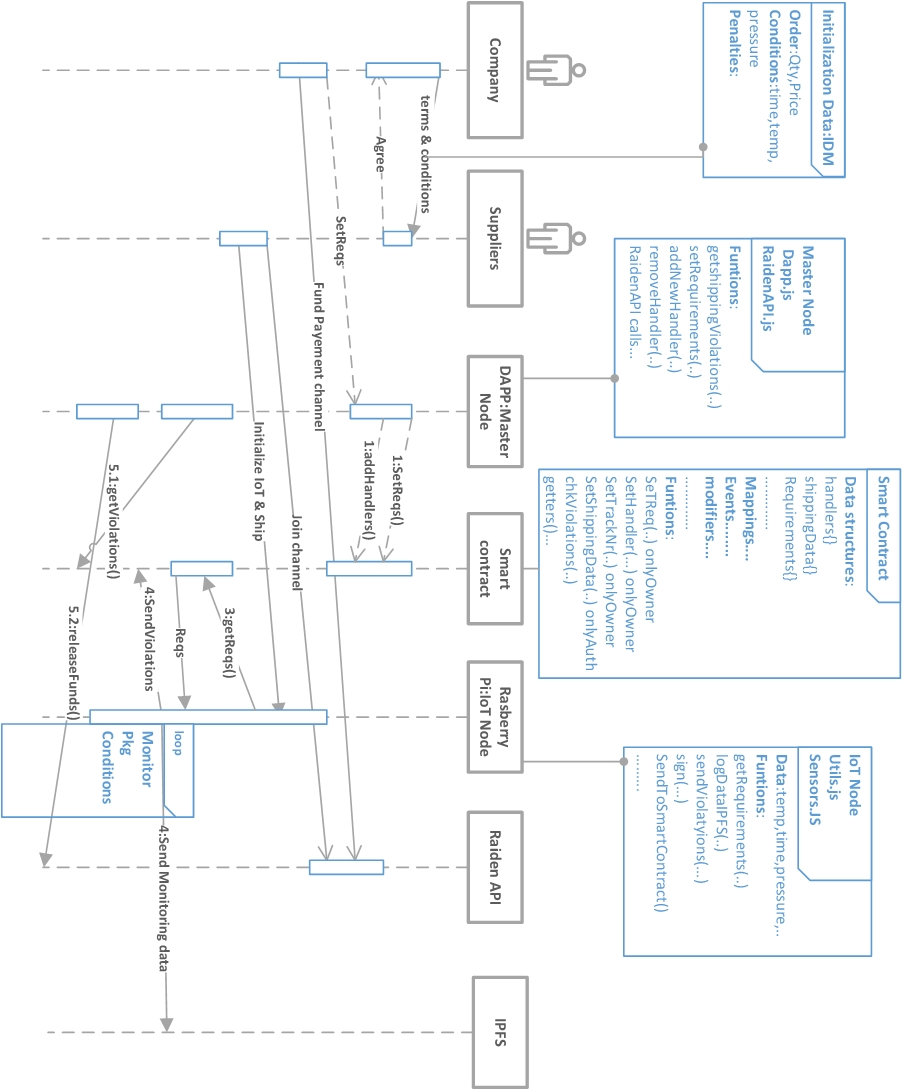
\includegraphics[width=180mm,scale=1]{figs/SD-Flip}
	\caption{Sequence diagram of the proposed package tracking system}
	\label{fig:SysSD} 
\end{figure}
\clearpage

\subsection{Hardware Setup}
\subsubsection{Master Node}
Master Node is implemented using NodeJS. All software dependencies are managed by node package manage i.e. NPM. This enables us to run the Master Node on any windows or Linux system capable of running NodeJS. Master Node sub-modules including Raiden and Geth are quite efficient in terms of RAM and CPU requirements. This enables us to run the Master Node on any moderately capable modern machine. As an example Master Node has been tested on a dual core virtual machine with a 4 GB RAM. There are however space constraints (HDD capacity) imposed due to the Raiden Network. Current iteration of Raiden requires that an Ethereum client must be running locally and fully synced with the blockchain. According to block explorer site “etherscan.io”, the current blockchain size of Ethereum main net is 98 GB, and of Ropsten test net is 50GB. Raiden Network team is currently working on an update which will enable users to sync with remote Ethereum nodes such as those provided by Infura. Until this update is ready the Master Node requires at least 60GB of free hard disk space to manage payment channels when deployed on Ropsten test net. 
\vspace{0.5cm}
\subsubsection{IoT Node}
The prototype IoT Node is shown in figure \ref{fig:piIoT}. It is implemented using a RaspberryPI 3 model B board, which is running Raspbian Stretch operating system. IoT node runs a custom package monitoring software solution, that is designed using NodeJS. We use GrovePi+ board to interface and connect Temperature, humidity, Light, and GPS sensors with the Raspberry PI.

\begin{figure}[h]
	\centering
    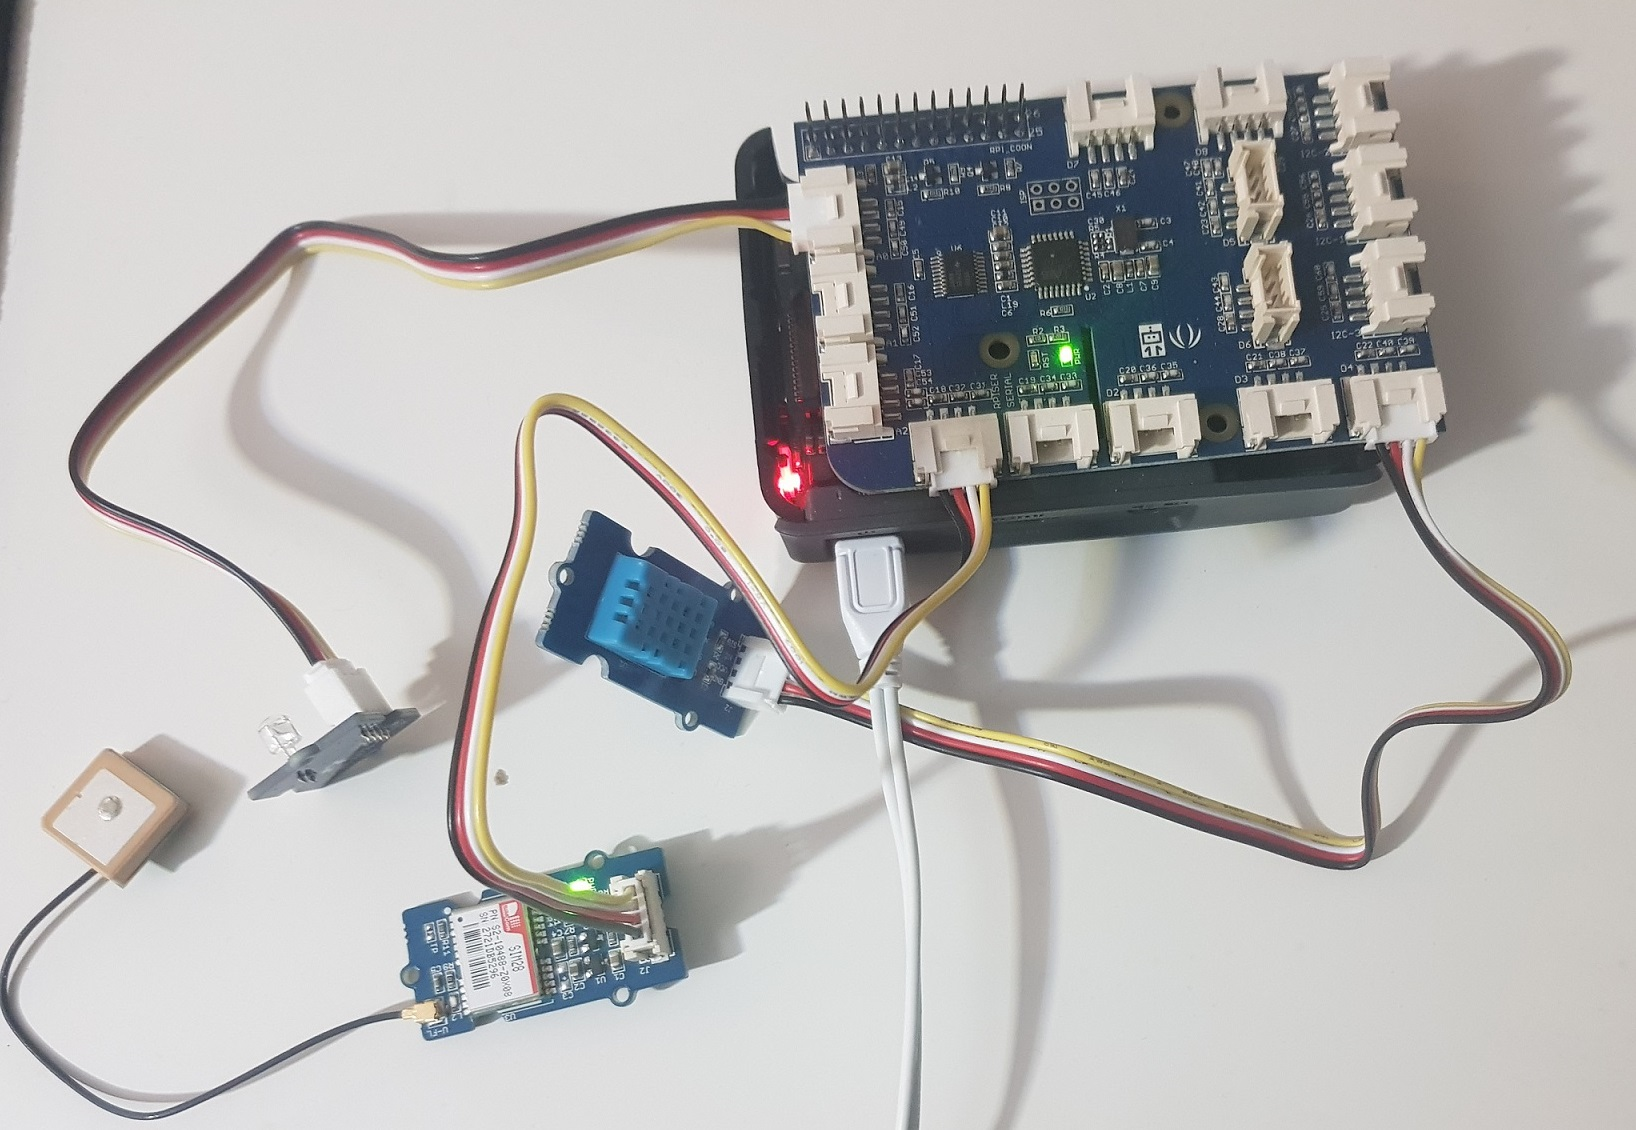
\includegraphics[width=140mm,scale=1]{figs/piIoT}
	\caption{Prototype IoT Node}
	\label{fig:piIoT} 
\end{figure}
\clearpage

%\subsection{Software Implementation}

\subsection{Master Node – Implementation} \label{IMN} 
The Mast Node has four sub modules as shown in its work flow diagram detailed in figure \ref{fig:master-workflow}. These modules are explained below:

\textbf{login:}
This is the first page that is presented to the user after starting the Master Node. It asks the user to provide the contract address of the Shipment Tracker contract. It also checks if the provided address is a valid Ethereum address. If the address is valid than Dapp.js module is called.

\textbf{MetaMask:}
MetaMask is a browser extension that enables users to communicate with decentralized applications deployed on Ethereum. It eliminates the need for users to run a local Ethereum node. It can be thought of as an Ethereum browser. MetaMask packages an Ethereum wallet, a Web3 injector and an Ethereum client all into one application. It enables our Dapp.js module to send signed transactions to the blockchain. It also manages identity of the user as it securely stores users public and private keys. The Dapp.js module queries MetaMask to get the public key for constant function calls.

\textbf{Dapp:}
This module provides the interfacing logic for communicating with the Shipment Tracker contract. Once loaded it first searched for the web3 library which in this case is injected by MetaMask. If Web3 library is not injected, then it looks for web3 and an Ethereum client on the local machine. The user can use the graphical user interface of this module to call functions from our Smart Contract. The contract ABI is packaged and stored with this module. There are two main types of functions in any Smart Contract i.e. constant functions and non-constant functions. The Master Node uses the MetaMask Ethereum client to get results of constant functions. Recall that constant functions do not alter any state in the blockchain. This is why they can be called without incurring any gas or fee. The remote Ethereum node simply executes these functions locally and returns the result to the Dapp module. This is shown in figure \ref{fig:master-workflow} with the decision box which checks if the transaction is a call to a constant function. State altering functions must be called through signed transactions. The Dapp module uses Web3 and contract ABI to prepare a transaction payload and then hands it over to the MetaMask. Which then prompts the user to confirm gas payment by signing the transaction. It then proceeds to broadcast the signed transaction to the Ethereum Network. The transaction is then mined and every node on the blockchain executes the Smart Contract function associated with the transaction.
%\clearpage
\textbf{RaidenAPI:}
Users can choose to load the RaidenAPI module any time after a successful login. This module presents the user with a unified GUI that shows all open channels. It allows consuming Raiden channels and payments endpoints from the RESTful API. The Raiden client must be running and fully synced for the API calls to be successful. The user is responsible for insuring that the client is running before starting this module. 

\begin{figure}[h]
	\centering
    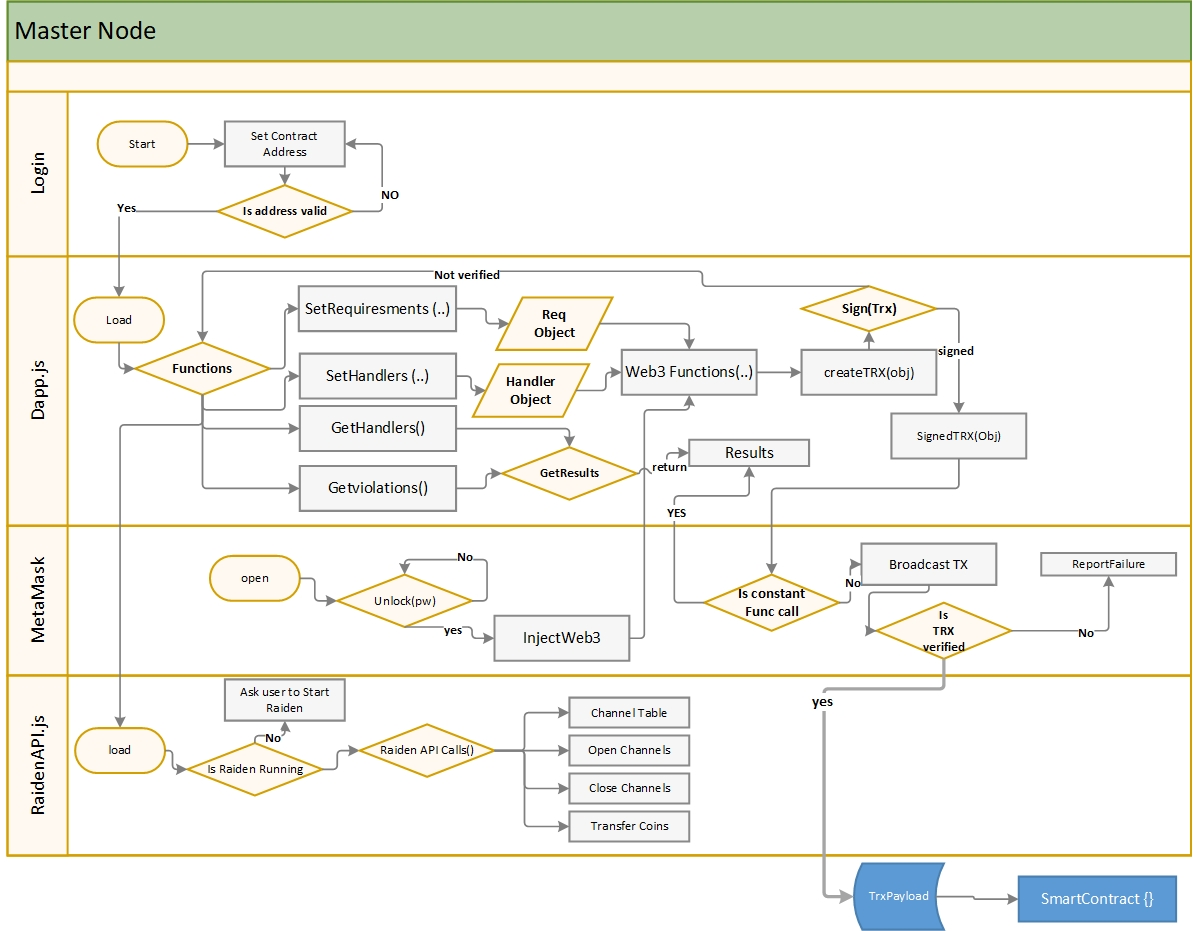
\includegraphics[width=175mm,scale=1]{figs/master-workflow}
	\caption{Work Flow diagram for Master Node}
	\label{fig:master-workflow} 
\end{figure}
\clearpage
\vspace{0.5cm}
\subsection{IoT Nodes – Implementation} \label{IoT-Nodes} 
The System work flow of IoT Node is shown in figure \ref{fig:IoTNode}. It is implemented as a command line program on RaspberryPI with the help of NodeJS. We have bundled all helper libraries including Web3.js, keyEthereum etc using node package manager utility. To start the shipping and monitoring process the supplier initializes the device with the tracking number. The device then contacts the SmartContract to read the shipping requirements associated with its tracking number. Transactions to Ethereum blockchain are relayed through remote Ethereum Nodes provided by Infura. It only provides API access to Ethereum nodes it does not store any keys nor does it handle transaction signing. The Sensors sub module calls functions in Utils modules to handle all Web3 calls. Utils module creates a web3 transaction to request a list of requirements the IoT Node need to adhere. This transaction is passed to Infura Ethereum Node which executes the request and returns results back to our node. Upon retrieving the shipping conditions from the Smart Contract the Sensors module initializes the required sensors i.e. temperature, light etc. Once the sensors have been initialized the IoT node enters the monitoring phase.  Monitoring is further divided into two phases: Checking for violations or Monitoring, and logging (shipment data).

\textbf{Monitoring:}
IoT Node checks sensor reading every few minutes to insure no violations have occurred. The monitoring period can be configured during initialization phase. If any violations are found, they are immediately sent to the Smart Contract to be recorded permanently. Violations are also added to the log. Recording violations in the blockchain is a state altering transaction, hence it must be signed by the Ethereum private key of the device. Utils module automates this process with the help of helper library ethereumjs-tx.js. Violations are signed with the Ethereum key of IoT Node and with the Post Quantum key of current shipper i.e. the one who breached the conditions. Violation packet sent to the blockchain is shown in figure \ref{fig:violation-impl}. The PQ key changes when a new shipper takes control of the package or shipping procedure.  Violation packets always carry the id of the current shipper along with the time and date of violations. This enables easy identification of the responsible party.

\textbf{Logging:}
Logging basically creates a detailed record of package conditions in the form of a log.  Each log entry contains the shipping data packet shown in figure \ref{fig:violation-impl}. In short logging function records sensor values, package location, and shipper ID every 5 minutes. This log is written to IPFS as a mutable file object. Utils appends new log chunks at the end of previous log stored at IPFS. The generated hash is stored in the blockchain. This allows retrieval of complete logs after package has been delivered. These logs are useful for analytics purposes. The IPFS log interval can be configured during the initialization phase. Logging and Monitoring continue as long as the package is in transit, and the shipping status remains un delivered.

\begin{figure}[h]
	\centering
    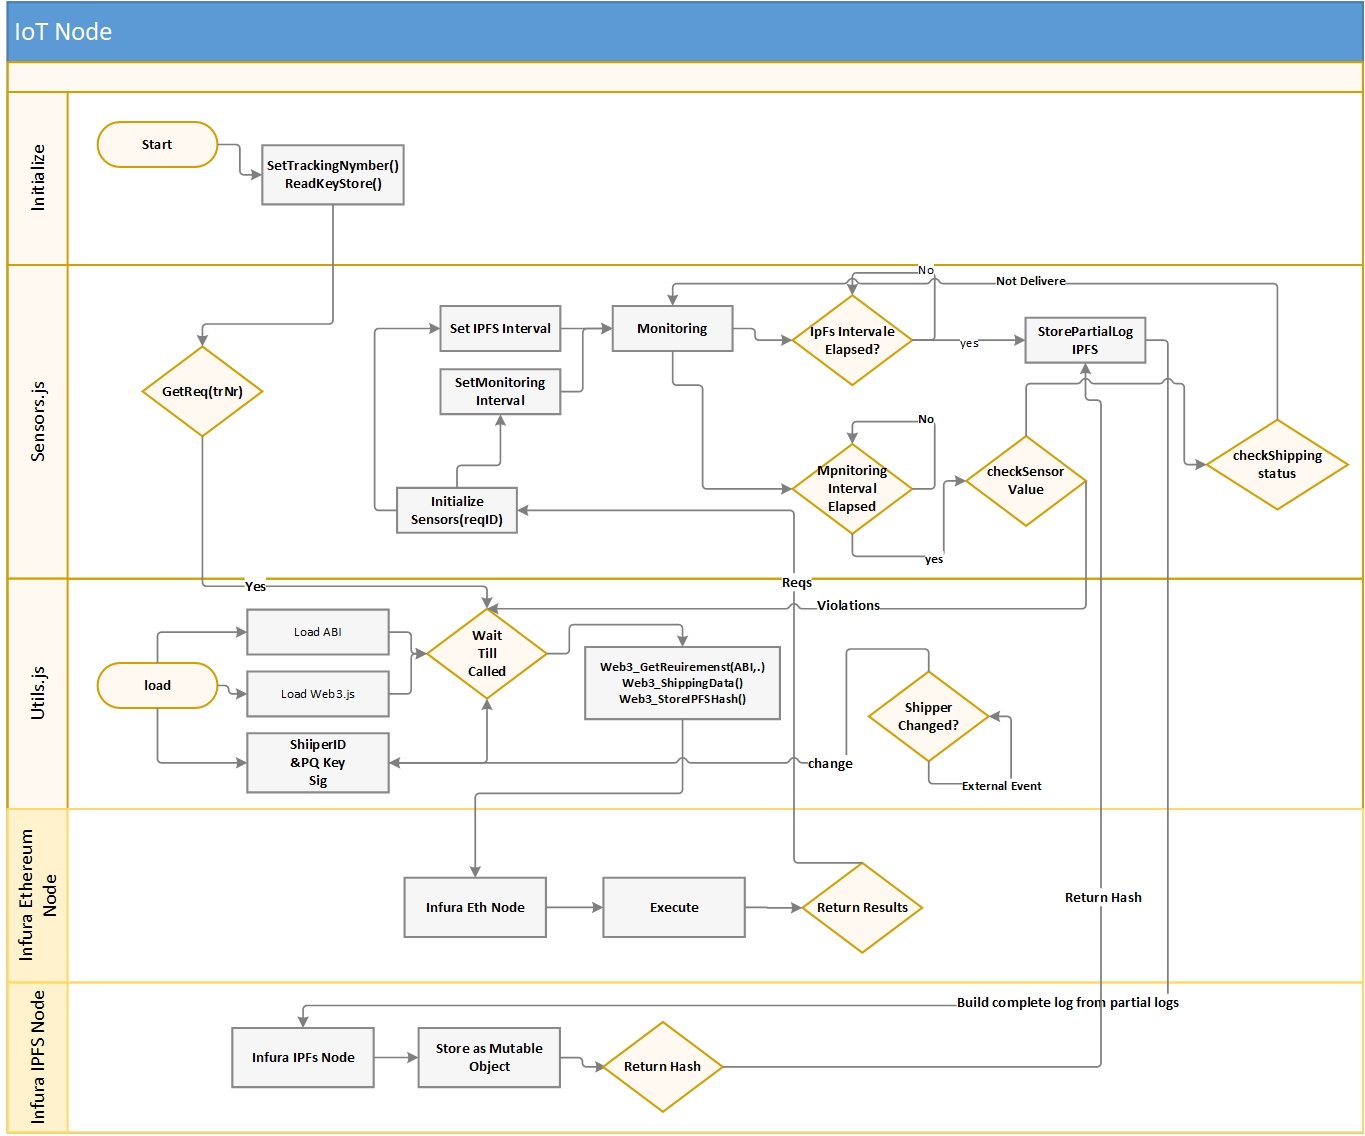
\includegraphics[width=180mm,scale=1]{figs/IoTNode}
	\caption{Work Flow diagram for IoT Node}
	\label{fig:IoTNode} 
\end{figure}
\clearpage

%\subsubsection{IPFS logging}

\subsection{Shipment Tracker – Design Details} \label{ST-SmartContract} 
This section presents important design elements of the Shipment Tracker Smart Contract. We have defined custom mapping and list structures to function as a logical database in our Smart Contract. This database saves tracking information, supplier access rights information, and shipping requirements. The primary key that logically binds different data structures is the tracking number. This tracking number is unique for each shipment or package. It is used as the key to store shipment data in the correct Solidity mapping. A mapping is a sort of hash table which is virtually initialized so that all possible keys exist in the table. In essence it is a key value pair mapping as shown in the figure \ref{fig:Sol-Mapping}. We have three main types of mappings in the Shipment Tracker contract. TrackingInfo mapping stores violations and tracking data associated with every package. This is described in \ref{SV}. HandlerList mapping defines the rights of IoT Nodes and shippers (see \ref{AuthHandlers}). It tells which handler or Node is able to send violations and data to be stored in the TrackingInfo mapping. RequirementList mapping is responsible for defining requirements according to which each individual package must be handled. Our design relies on custom defined Solidity Modifiers that prevent shippers and IoT Nodes from modifying unauthorized sections of the database. Function modifiers are explained below:

\begin{figure}[h]
	\centering
    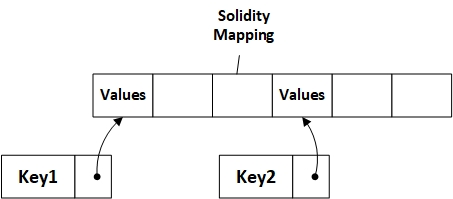
\includegraphics[width=110mm,scale=1]{figs/Sol-Mapping}
	\caption{Sample Solidity Mapping}
	\label{fig:Sol-Mapping} 
\end{figure}

\textbf{Function Modifiers}

Modifiers are a convenient way to modify a functions behavior. They make sure that certain conditions are met before a contract function is executed. They are most commonly used to restrict access to certain parts of the program. When a function is called its modifiers are executed first to decide if the calling user or private key has the right to read or change the contract state. Shipment Tracker contract has three main modifiers as shown in figure \ref{fig:sc-workflow}. They are described in \ref{CWF}. Together these three modifiers perform authorization checks on different functions of the smart contract.
\clearpage

\subsubsection{Shipment Tracker – Contract Work Flow} \label{CWF}
The functionality of the important sub modules of the Smart Contract are explained in the diagram presented in figure \ref{fig:sc-workflow}. The AuthorizeHandlerAddress function stores the IoT Node’s Ethereum public key and Shippers ID and PQ keys. This data is stored as Handler Object in the HandlerList mapping. This mapping uses the tracking number as keys. Each key in the mapping corresponds to a dynamic list of handler objects as shown in figure \ref{fig:handler-impl}. This function also insures that handler objects in all handler lists are unique. CheckAuthorization is the combination of two modifiers i.e. “onlyOwner” amd “onlyAuthorized”. The first modifier insures that only the contract owner i.e. the person in possession of the private key that deployed the contract, can make certain types of changes. This modifier is used for defining requirements on individual packages as explained in section \ref{SV}. The company is the only party that is able to define package requirements in the Smart Contract. “onlyAuthorized” modifier insures that shipping data and violations sent from IoT Nodes are saved in the correct section of the TrackingInfo mapping. It prevents unauthorized devices from modifying this mapping. The VerifySignature function shown in the diagram performs Post Quantum signature verification on the data received from the IoT Node. "OnlyIfSigMatch" modifier uses this function to insure that data and violations sent to the blockchain are correctly signed by the shippers PQ key. This insures data integrity. It insures that correct party could be held accountable for violations. This is particularly important in the cases where there is more than one shipper involved in the shipping procedure. To send violations to the blockchain IoT nodes call the LogTrackingInfo contract function. IoT Node sends current shippers ID in plain text form along with violations. Violations are encrypted and signed by the shippers PQ key. LogTrackingInfo uses the unencrypted shipper ID to locate shippers PQ key stored in the HandlerList mapping. It than proceeds to decrypt the encrypted information and calls the ChkViolation function. This function checks if the tracking data sent to contract is a violation according to the defined requirements. Once a requirement violation is verified it stores it in the TrackingInfo mapping and fires the violation event. Master Node and shippers can subscribe to violation events to get critical real time information related to package conditions. There are several Get Functions defined in the contract to read stored information related to a package. These include functions to read list of shippers authorized to handle the package, requirements according to which this package should be handled, and any and all violations incurred during shipping process. Finally, IoT node uses the SetIPFS function to store IPFS hash address of the detailed log created during shipping. This log can be retrieve from anywhere just by knowing the hash address.      
\clearpage   
\begin{figure}[h]
	\centering
    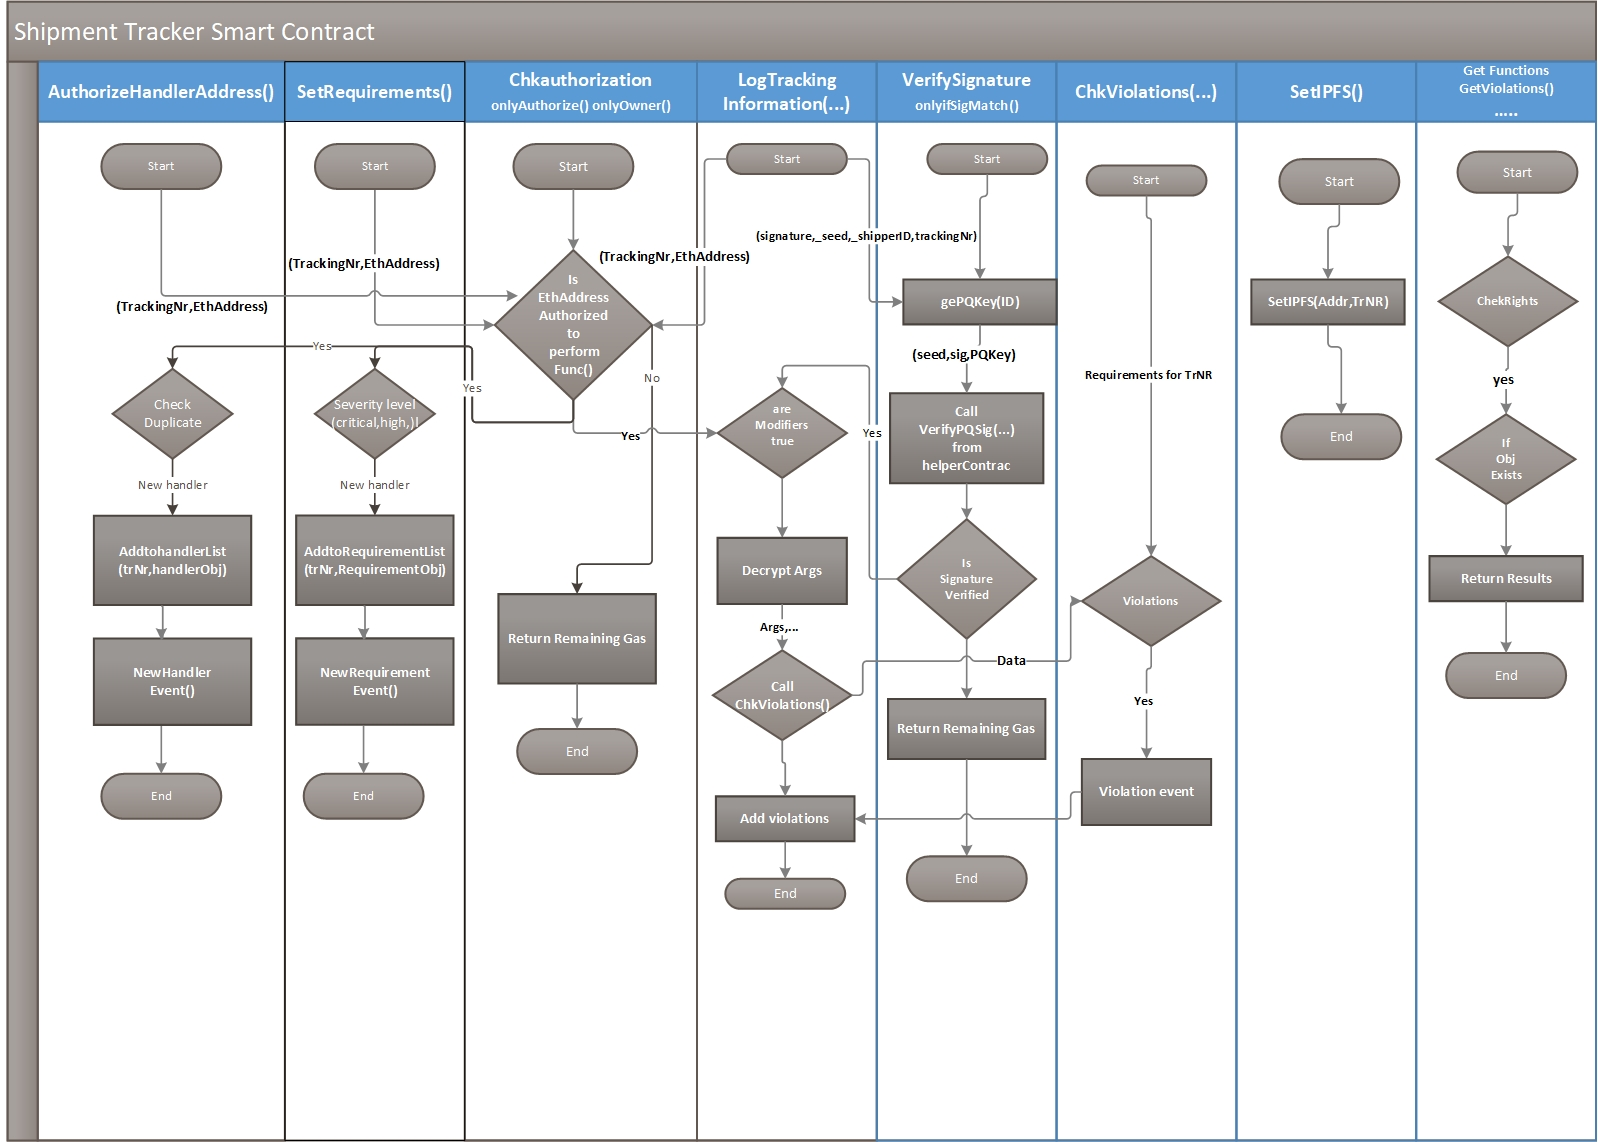
\includegraphics[width=175mm,scale=1]{figs/sc-workflow}
	\caption{Shipment Tracker work flow}
	\label{fig:sc-workflow} 
\end{figure}
\vspace{0.5cm}

\subsubsection{Handler Authorization} \label{AuthHandlers}
The AuthorizeHandlerAddress (see fig \ref{fig:sc-workflow}) allows Shippers and IoT Nodes to communicate shipping data and violations with the Smart Contract. Each package has one or more handlers or shippers who are authorized by the company to handle packages during shipping. The list of authorized handlers is stored in the HandlerList mapping shown in figure \ref{fig:handler-impl}. This mapping uses the tracking number of the package to create a dynamic list of handler objects. Each handler object represents only one shipper. Each object contains the shipper ID, their PQ key and the IoT Node Eth address. The IoT nodes Eth address is used for communicating shipping data with the blockchain. The company adds shippers or handlers to the HandlerList mapping by generating a transaction using the Master Node’s graphical interface. This is a state altering operation; hence it must be signed using company’s private Ethereum key. Contract design dictates that this key must be the same as the one that was used to deploy the Shipment Tracker Contract. This key is represented as Master Node Eth Address in the figure \ref{fig:handler-impl}. 
\clearpage


\begin{figure}[h]
	\centering
    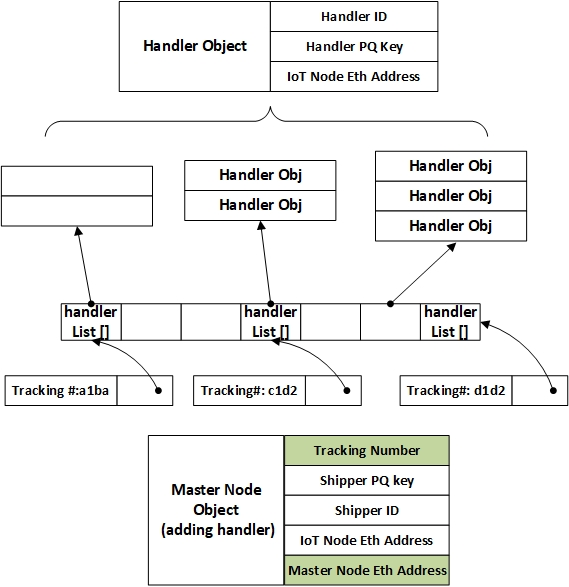
\includegraphics[width=120mm,scale=1]{figs/handler-impl}
	\caption{Adding a new handler to the Handler List}
	\label{fig:handler-impl} 
\end{figure}
\vspace{0.1cm}
\textbf{Revoking Authorization}

If for any reason the company wishes to revoke the authorization of a shipper. They can do so by calling RevokeAuthorization function using the Master Node. This function removes the handler object associated with the shipper in the handler list. This is also a state changing operation and as such must be completed using a signed transaction.

\vspace{0.5cm}
\subsubsection{Requirements}
Setting Shipping Requirements is similar to authorizing handlers as evident from the work flow diagram in figure \ref{fig:sc-workflow}. Adding or removing requirements is a state changing operation and as such can only be executed using signed transactions. A miner verifies that the transaction is correctly signed by company’s private key. It then passes the transaction payload to the Smart Contract. The transaction payload in this case is a call to SetRequirements function of the Shipment Tracker Contract. The contract verifies weather the Ethereum address that made this call has the right to execute this function. This is achieved using the “onlyOwner” function modifier.  The SetRequirements function parses the received Master Node object shown in figure \ref{fig:requirement-impl} and extracts the tracking number. This tracking number is the key for storing requirements in the RequirementsList Mapping. The function then creates the Requirement object. This object is saved in the dynamic array that corresponds to the tracking number in the mapping as shown in figure  \ref{fig:requirement-impl}. The requirement object can hold different types of requirements e.g temperature, light, pressure, Humidity etc. This necessitates that the requirement object is as generic as possible. This object has two essential properties i.e. requirement ID and Severity Level. Everything else is optional. Requirement ID uniquely identifies a type of requirement e.g. temp for monitoring package temperature. Severity level can have one of four values e.g. Critical, High, Medium and Low. Max Threshold and Min Threshold properties of the requirement object define the maximum and minimum values that must never be exceeded. As an example consider a medical substance that must be transported under strict climate controlled conditions. The package temperature must never exceed $25^\circ$C (Max Threshold), neither should it fall below -$10^\circ$C (Min Threshold). there could be conditions that only require one type of threshold i.e. either max or min. The two requirement flags i.e. Min Flag and Max Flag enable the IoT node to determine, which threshold is relevant for any given requirement ID. If both flags are true than then it checks the sensor values against both thresholds.  
\vspace{1mm}
\begin{figure}[h]
	\centering
    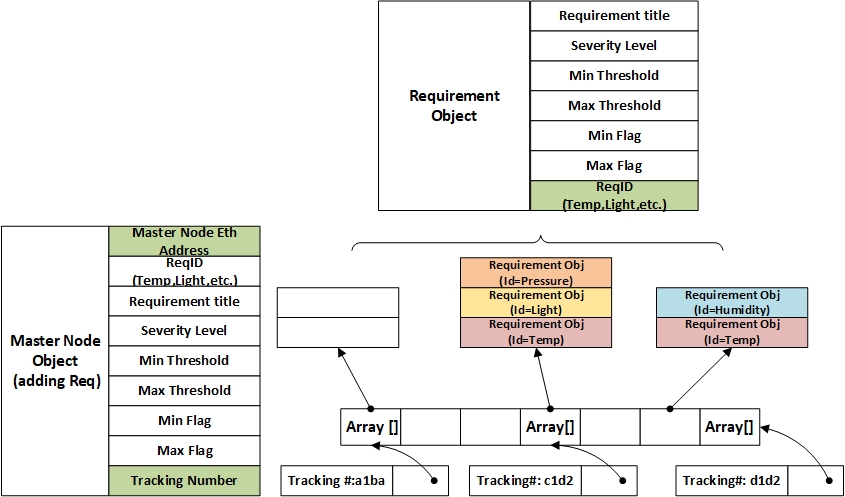
\includegraphics[width=170mm,scale=1]{figs/requirement-impl}
	\caption{Setting shipping requirements for a package}
	\label{fig:requirement-impl} 
\end{figure}

\textbf{IoT Nodes and Requirements:} 
IoT Node requires a set of requirements to begin monitoring package conditions. It receives these requirements by sending its tracking number in the form of a get request to the Shipment Tracker contract. The contract responds to IoT node’s request by sending all the requirements associated with a particular tracking number. This requirement ID determines which environmental conditions the IoT Node will monitor. These nodes have been tested with temperature, humidity, pressure, and GPS sensors. Additional sensors can be easily integrated without requiring any major changes to the design. %In the Master Node this is simply a matter of defining additional requirement IDs. The IoT Node reads the requirements and checks if it has a sensor capable of monitoring the conditions defined by the requirement ID. If no such sensor is found it proceeds to the monitoring phase, but only monitors the condition for which it has sensors for.
\vspace{0.5cm}
\subsubsection{Violations} \label{SV} 
IoT nodes are responsible for monitoring shipping conditions according the defined requirements during shipping. Each shipping cycle is logically separate from others. It could be that an organization has different set of suppliers for different products. IoT nodes and suppliers only have access to the parts of the database (mappings) that are associated with their package tracking number as shown in figure \ref{fig:violation-impl}. This insures that shipment data and violations remain logically separated even with multiple parallel supply lines. The shipping data object sent from the IoT Node has the tracking number, which is used as the key in the Solidity mapping as shown in figure \ref{fig:violation-impl}. This object is signed with the post quantum key of the shipper. This insures data integrity even in the presence of Post Quantum threats. IoT Node can be optionally configured to encrypt certain parts of the shipping data object to protect confidentiality during transit. Shipment Tracker contract parses the received shipping data object and creates the violation object shown in figure \ref{fig:violation-impl}. This object is passed to the check violations functions and to confirm shipping violations and to fire appropriate violation events. Company and suppliers can subscribe to these events and respond in real time. All violations are permanently stored on the blockchain.
\vspace{0.1cm}
\begin{figure}[h]
	\centering
    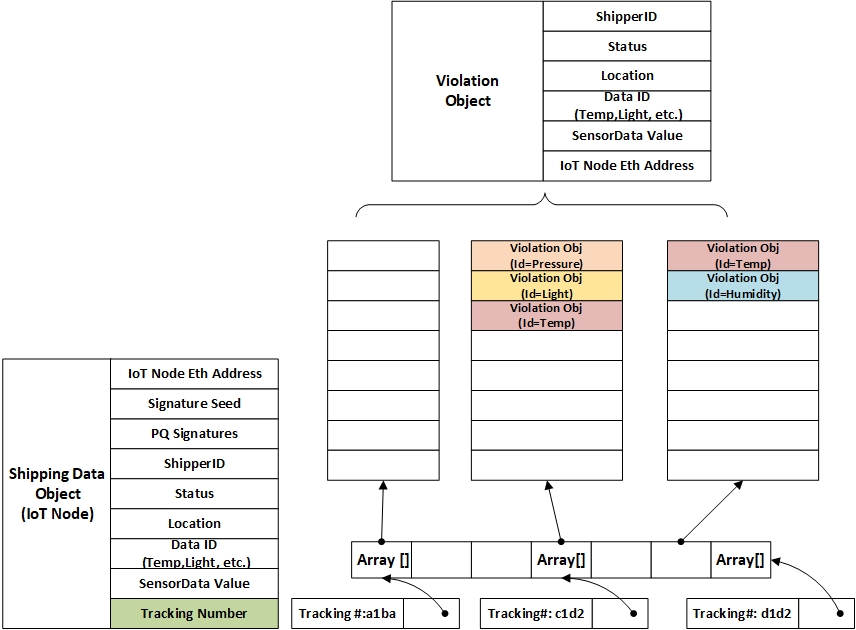
\includegraphics[width=160mm,scale=1]{figs/violation-impl}
	\caption{Adding shipping data and violations to the blockchain}
	\label{fig:violation-impl} 
\end{figure} 
\clearpage
\subsection{Securing the System against Post Quantum Adversaries}
The biggest advantage of a blockchain is the security benefits afforded to them due to their decentralized nature. Blockchain security model relies on a combination of cryptographic primitives, secure hashing algorithms, digital signatures and distributed nodes. It is almost impossible for a single attacker to hack the blockchain. Relying on traditional means any successful attacker would need to control more than half the nodes or network hashing power to create fraudulent transactions. This is known as a 51 percent attack. This attack is almost impossible in large blockchain networks such as Bitcoin and Ethereum. However, one thing that could pose a threat to blockchain are Quantum Computers. They are a promising area of research, but could one day prove to be an existential threat to the blockchain. This is because they can at least in theory break the cryptographic primitives that blockchains rely on. One of our goals is to design a system with architecture primitives that could defend against any future quantum adversaries. It needs to prevent attackers from modifying critical parts of the system such as violation data. This system can be explained with the help of algorithm \ref{alg:MYALG}.  

Our proposed security model relies on a combination of rights management based on Solidity modifiers and post quantum algorithms for generating secure digital signatures. Important parts of this solution are explained in detail in section \ref{ST-SmartContract}. The post quantum signature scheme for this scenario uses lattice based algorithms developed at TU Darmstadt such as \cite{cryptoeprint:2011:484}. Alternatively, we can also use schemes recently submitted to NIST. The PQ algorithm is implemented in a separate library contract as shown in figure \ref{fig:ArchitectureSC}. Our Shipment Tracker contract uses a wrapper function to call the signature verification function of the helper contract. This enables us to easily change the post quantum algorithm without requiring any major changes in the Shipment Tracker Contract. This security model only protects data integrity, additionally it can be used to protect confidentiality during transport. We can not guarantee confidentiality of data once it has been stored on the blockchain.  This is because everything stored on the blockchain is by default visible to every node having a copy of the ledger. A malicious node can dig through the stored blocks and get PQ keys of authorized shippers using eth.getStorageAt function. They can then use these keys to decrypt data. %If we use asymmetric post quantum algorithm than knowing the PQ public key alone will not be enough to violate integrity. 

\begin{algorithm}[!h]
  Initialize the IoT device\;
  \KwData{Get Sensor Data}
 \While{Shipping status not Delivered}{  
  Check violations\;
  \eIf{violation detected}{
   Start signature procedures\;
   Seed = random(256)\;
   PQSign = Sign(Message,SecretKey)\;
   message = (dataID || location || status ||TimeStamp)\;
   Encrypt function arguments\;
   TrxPayload =     Functioncall(encryptedArg1,encryptedArg2,...,PQsign,TimeStamp,shipperID)\;
   CreateSignedEthTransaction(EthpvtKey,TrxPayload)\;
   BroadcastTransaction\; 
   save violation and shipping data in IPFS;	

   }{
   save shipping data in IPFS\;
  }
 }
 Blockchain verifies GAS and Ethereum Signatures\;
 \While{Miners available} {
 checkAuthorization(IoTNode public key)\;
 get shipper PQ key from Shipper ID\;
 Smart contract verifies PQ signatures\;
 \eIf{Verify(PQkey,TimeStamp,signature)}{
  	\eIf{(Eth Signatures Authorized and PQ Signatures Authorized)}{
  		message = DecryptArguments(cArg1,cArg2,...)\;
  		execute the function\;
  		fire Events\;
  	}{
  		Return Error\;
  	}
  	

   }{
   Return Error\;
  } 
 
 }
\caption{System Security Model Algorithm}
\label{alg:MYALG} 
\end{algorithm}
\clearpage



\subsection{Implementation Challenges}
\subsubsection{Problems with Raiden and Fixes}
We faced most difficulties while getting Raiden client to work reliably. When we started developing our solution Raiden was in its developer preview / beta stage. We choose it because at that time it was the most mature off chain transaction solution available for the Ethereum Echo system. The other solutions under consideration was Perun, which at the time was still working on a proof of concept implementation. Raiden was particularly difficult to setup and get off the ground. To get started it first needs to completely sync with the Ethereum blockchain. This process can take up to 3 to 5 days to complete in the worst case scenario. Even after syncing it required that the machine hosting Raiden remained on to as continue syncing with new transactions. If we turned off the machine, we would have to wait for it to catch with the blockchain before we could use it again.   Once it was setup we faced further problems making direct payment transfers. The direct payments worked intermittently.  This problem led us to contact the Raiden team to find a solution. We worked closely with the development team to debug the issue. It was concluded that the Raiden Nat punching module was the culprit. This module is required to punch through firewall and local Nat routers. This module did not always work reliably. In order to make direct payment transfer Raiden nodes need to be able to ping each other. In the end we found a work around which worked 90 percent of the time. At the time of last contact Raiden developers were still working on a permanent fix for the Raiden Nat punching module. Raiden has now also updated its official documentation \cite{rad:001} to add a set of best practices to be implemented by the user. These best practices are closely aligned with the work around that we discovered to resolve some of the situations we were facing.
%\clearpage
\vspace{0.5cm}
\subsubsection{Problems with Web3}
The Web3 is a JavaScript helper library which allows us to communicate with Ethereum nodes over HTTP connections. In our project we use node package manage NPM to manage dependencies for us. NPM always installs the latest official version of the required libraries. When we started development the latest version was Web3 0.20.6. Half way through development a new version of the Web3 library i.e. 1.0.0 was released. The new update radically overhauled how the library was implemented and worked. It changed functional interfaces and how they are called. The new update also changed the manner in which the functions could be used by making major architectural changes in Web3 function calls. This forced us to re-implement and overhaul application code for Master Node and IoT Node. In version 0.20.6 a Web3 function calls behaved synchronously i.e. execution of the module would halt until the call was resolved. This meant we could count on the next function to always get correct results from the previous function calls. In the new 1.0 update Web3 function calls behave asynchronously i.e. it does not halt any part of the program. This means that after a transaction call was made it would return immediately and return control to the next function inline even though the previous function has not resolved yet. Instead of returning values new update returns JavaScript Promises. This means we are required to use callbacks to resolve promises correctly. We also had to re design how we passed values from individual sub modules to other modules. In version 0.20.6 we passed the values directly to other modules, in version 1.0.0 we had to redesign IoT Node sub modules to use Async/Await for communicating values across module boundaries.  

